\documentclass[pagesize=pdftex,paper=a4,bibliography=totoc,listof=totoc,12pt]{scrreprt}

%%%%%%%%%%%%%%%%%DATEN%%%%%%%%%%%%%%%%%
%Erstellungsdatum
\date{\today}

%%%%%%%%%%%%%%%%%pakete%%%%%%%%%%%%%%%%%
% böses hackpaket
\usepackage{scrhack}

%neue Rechtschreibung
\usepackage[ngerman]{babel}
\usepackage{babelbib}
 
%\usepackage[T1]{fontenc}
%Umlaute ermölichen utf8 ( latin1)
\usepackage[utf8]{inputenc}
 
% Tabellen
\usepackage{array}
 
% Schriftfarben
\usepackage{color}

% FloatBarrier
\usepackage{placeins}
%Bilder
\usepackage{float}
\usepackage{floatflt}
\usepackage[pdftex]{graphicx}
\usepackage{caption} %für subfigure
\usepackage{subcaption} % für subfigure
\DeclareGraphicsRule{*}{mps}{*}{}
%\usepackage{PSTricks}

%Math
\usepackage{amsmath}
% bessere theorem umgebung als amsthm (zeilen umbruch nach überschritf und aufzählung)
\usepackage[amsmath, thmmarks]{ntheorem} 
\usepackage{amssymb}
\usepackage{mathrsfs} % \mathscr command for categories
\usepackage[all]{xy} % Kommutative-Diagramme

% Pseudocode in latex
\usepackage{algorithm2e}

%Nomenclature
\usepackage[intoc]{nomencl}

%Kopf-/Fußzeilen
\usepackage{fancyhdr}

%Hyperref für Bookmarks im PDF
\usepackage[pdftex, pagebackref]{hyperref}

%%%%%%%%%%%%%%%%%%%%seitencfg%%%%%%%%%%%%%%%%%%%%%%%%%%%%
\pagestyle{fancy}
\fancyhf{}
%Kopfzeile links bzw. innen
\fancyhead[L]{\nouppercase{\leftmark}}
%Kopfzeile rechts bzw. außen
\fancyhead[R]{\thepage}
%Linie open
\renewcommand{\headrulewidth}{0.5pt}
%Fußzeile links bzw. innen
\fancyfoot[L]{Hausarbeit Simulation}
%Fußzeile rechts bzw. außen
\fancyfoot[R]{\today}
%Linie unten
\renewcommand{\footrulewidth}{0.5pt}

% Chapterstyle
\usepackage[Sonny]{fncychap}

\hypersetup {
pdftitle = {Verkehrsflusssimulation einer Kreuzung},
pdfsubject = {Hausarbeit Simulation}, 
pdfauthor = {Julian Berndt, Hannah Dusch, Martin Kraus, Philipp Schwarz},
pdfhighlight = {/O},
pdfkeywords = {Nagelschreckenberg, Kreuzung, Verkehrssimulation, Fundamentaldiagramm}, colorlinks = {false},
bookmarksnumbered = {true},
citebordercolor = {1 1 1},
linkbordercolor = {1 1 1},
urlbordercolor = {1 1 1},
bookmarksopen = {true},
bookmarksopenlevel = {1}
}

% Nummerierungen bei Aufzählungen (Erste Ebene Römisch) 
\renewcommand{\theenumi}{\roman{enumi}}
\renewcommand{\labelenumi}{\theenumi)}

%%%%%%%%%%%%%%%%%%%EIGENE-BEFEHLE%%%%%%%%%%%%%%%%%%%%%%%%
\newcommand{\ncl}[2]{\nomenclature{\textit{#1}}{\textcolor{white}{test}\\#2}}
\newcommand{\glossar}[1]{\textit{#1}\glossary{\textit{#1}}}

%Bilder
\newcommand{\pic}[1]{Abbildung \ref{#1}}
\newcommand{\picp}[1]{Abbildung \ref{#1} Seite \pageref{#1}}
%Tabellen
\newcommand{\tab}[1]{Tabelle \ref{#1}}
\newcommand{\tabp}[1]{Tabelle \ref{#1} Seite \pageref{#1}}
%Darstellung eines Links im Quellenverzeichnis
\newcommand{\urlg}[2]{\url{#1}\\zuletzt abgerufen am #2}
%Verweise
\newcommand{\see}[1]{(siehe Kapitel \ref{#1})}
\newcommand{\seeo}[1]{siehe Kapitel \ref{#1}}
\newcommand{\seea}[1]{(siehe Anhang \ref{#1})}
\newcommand{\refThmIt}[1]{\textit{\ref{#1})}}
% Fett und Schief
\newcommand{\textbit}[1]{\textbf{\textit{#1}}}
%\newcommand{\beweis}{\textbf{Beweis:} }
%\newcommand{\qed}{\hfill \(\square\)}
%\newcommand{\noteH}{\textbf{Bemerkung:} }
\newcommand{\defH}[1]{\underline{#1}}

\newcommand{\code}[1]{\texttt{#1}}

% theoremartige Konstrukte
%-------------------------
% diese haben keinen zeilenumbruch nach d. Überschrift
\theoremstyle{plain}
\newtheorem{Def}{Definition}[chapter]
\newtheorem{Satz}{Satz}[chapter]
\newtheorem{Korollar}{Korollar}[chapter]
\newtheorem{Lemma}{Lemma}[chapter]

% Jetzt mit Zeilen umbruch nach Überschrift 
% (Counter aber von obigen Konstrukten benutzen)
\theoremstyle{break}
\newtheorem{Def-break}[Def]{Definition}
\newtheorem{Satz-break}[Satz]{Satz}
\newtheorem{Korollar-break}[Korollar]{Korollar}
\newtheorem{Lemma-break}[Lemma]{Lemma}

% Bemerkungen
\theoremstyle{plain}
\theorembodyfont{\normalfont}
\theoremseparator{ :}
\newtheorem{Bem}{Bemerkung}[chapter]

% Beispiele
\theoremstyle{plain}
\theorembodyfont{\normalfont}
\theoremseparator{ :}
\newtheorem{Bsp}{Beispiel}[chapter]

% Eigene beweisumgebung
\theoremstyle{nonumberplain}
\theoremheaderfont{\itshape}
\theorembodyfont{\normalfont}
\theoremseparator{.}
\theoremsymbol{\ensuremath{\square}}
\newtheorem{proof}{Beweis}
\newtheorem{proofsketch}{Beweisskizze}
% Fix für die Beweisumgebung:
% Steht vor \end{proof} ein \end{align}, so wird das 
% qed-symbol nicht so schön gesetzt: \mbox{} einfügen
%-----------------------------

% mathebefehle
%-------------
\DeclareMathOperator{\Hom}{Hom} % Klasse der Morphismen einer Kategorie
\DeclareMathOperator{\Morph}{Morph} % Klasse der Morphismen einer Kategorie
\DeclareMathOperator{\Obj}{Ob} % Klasse der Objekte in der Kategorie
\DeclareMathOperator{\id}{id} % Identische Abbildung / Morphismus
\DeclareMathOperator{\mod1}{(mod\mbox{ }1)} % mein Modulo-Operator
\DeclareMathOperator{\modk}{(mod\mbox{ }n)} % mein Modulo-Operator
\DeclareMathOperator{\diverg}{div} % Divergenz
\newcommand*\rfrac[2]{{}^{#1}\!/_{#2}} % schönere Brüche (Schiefes bruchzeichen)
\newcommand{\sprod}[2]{ \left\langle #1 , #2 \right\rangle } % skalarprodukt
\newcommand{\dcup}{\mathbin{\dot{\cup}}} % Disjunkte Vereinigung
\newcommand{\dbigcup}{\mathbin{\dot{\bigcup}}} % Disjunkte Vereinigung
% Kategorien
\newcommand{\Ens}{{\mathscr{E}\!ns}} % Kategorie der Mengen
\newcommand{\Top}{{\mathscr{T}op}} % Kategorie der topologischen Räume
\newcommand{\Mess}{{\mathscr{M}\!ess}} % Kategorie der Messräume
\newcommand{\Mass}{{\mathscr{M}\!ass}} % Kategorie der Messräume
\newcommand{\Ban}{{\mathscr{B}an}} % Kategorie der Bannachräume
\newcommand{\Hil}{{\mathscr{H}il}} % Kategorie der Hilberträume
\newcommand{\Dyn}{{\mathscr{D}yn}} % Kategorie der dynamischen Systeme
\newcommand{\Mdyn}{{\mathscr{M}\!dyn}} % Kategorie der maßtheoretischen dynamischen Systeme
\newcommand{\Tdyn}{{\mathscr{T}\!dyn}} % Kategorie der topologischen dynamischen Systeme
%\newcommand{\Ban1}{{\mathscr{B}an_1}} % Kategorie der Banachräume (Isometrien)

%\newcommand{\comp
%\newcommand{\comp}[1]{{#1}^{c}} % Mengenkomplement
%\newcommand{\compm}[2]{{#1}^{c(#2)}} % Mengenkomplement mit Grundmenge
%\newcommand{\compm}[2]{{#1}^{c\mathsf{[}#2\mathsf{]}}} % Mengenkomplement mit Grundmenge
%\newcommand{\compm}[2]{{#1}^{\complement\tiny{#2}}} % Mengenkomplement mit Grundmenge

%%%%%%%%%%%%%%%%%%%%NOMENCLATURE/GLOSSAR%%%%%%%%%%%%%%%%%%%
%Nomenclature 
\makenomenclature

%Glossar
%\include{glossar}

%%chemie
%\usepackage[version=3]{mhchem}

%own commands
%Merkbox:
%\begin{merkbox}
% text
%nomenclature}
% \newsavebox\TBox
% \newenvironment{merkbox}
%{%\par\noindent
% \begin{lrbox}{\TBox}
% \varwidth{\textwidth-2.5\fboxsep}
% }{\endvarwidth\end{lrbox}%
% \textcolor{orange}{\textbf{Merke:}}\\[1mm]
% \Ovalbox{\usebox\TBox}\par
%}

%markierungen
%\newcommand{\texthigh}[1]{\textcolor{orange}\textbf{#1}}
%\newcommand{\texthead}[1]{\emph{#1:}\hline}


\begin{document}
\pagenumbering{roman}
%Titelseite
%Titlepage und Logo
\begin{titlepage}

\titlehead{
  \centering
  \Large 
  \textbf{Ostbayerische Technische Hochschule Regensburg \\ Fakultät für Informatik und Mathematik}\\
   \vspace{2cm}     
	 
\includegraphics[width=8cm]{0_logo.jpg}
   \title{Hausarbeit im Fach Simulation}
   \subtitle{Verkehrsflusssimulation einer Kreuzung durch ein angepasstes Nagel-Schreckenberg-Modell}
	 \author{Julian Berndt, Hannah Dusch, Martin Kraus, Philipp Schwarz}
	 \vspace{2cm}
}
\date{\today}

\maketitle

\end{titlepage}


\newpage

%Inhaltsverzeichnis
\tableofcontents
%Abbildungsverzeichnis
\listoffigures
%\addcontentsline{toc}{chapter}{Abbildungsverzeichnis}
%Tabellenverzeichnis
%\listoftables
%\addcontentsline{toc}{chapter}{Tabellenverzeichnis}
\newpage

\pagenumbering{arabic}
% Die einzelnen Kapitel
\chapter{Einleitung}

\section{Aufgabenstellung}\label{sec:aufgabenstellung}

\section{Umsetzung}
TODO kurz beschreiben was wir gemacht haben (um die aufgaben zu
bwältigen wurde ein matlabprogramm erstellt mit dem sich ...) etc.

% - Aufgabenstellung
% - Umsetzung (kurz was gemacht wurde)
\chapter{Modellierung}

\section{Nagelschreckenberg Model}
Bei der Modellierung des Straßenverkehrs gibt es verschiedene Ansätze. Je nachdem welche Fragen mit dem Modell beantwortet werden sollen, bzw. worauf man bei einem Modell Wert legt, fällt die Wahl des Modells aus. Bei der makroskopischen Simulation eines Verkehrsflussproblems wird der Straßenverkehr global betrachtet, als fließende Bewegung, die hinsichtlich kollektiver Größen ausgewertet wird. Die Analyse des Modells erfolgt mithilfe von Geschwindigkeit und Dichte des Flusses. Möchte man die einzelnen Fahrzeuge betrachten und dabei die Anzahl pro Zeiteinheit oder die Dichte pro Strecke auswerten, so bietet sich der mikroskopische Simulationsansatz an, welches auch bei der Simulation der Kreuzung verwendet wurde. \\
\\
Die Grundlage bei der mikroskopischen Simulation des Verkehrsflusses bildet das sogenannte Nagelschreckenberg Model. Dieses wurde nach Kai Nagel und Michael Schreckenberg benannt, die das Verkehrsmodell mithilfe der Theorie der zellulären Automaten entwickelt haben, siehe \cite{article:NaSch}. \\
\\
%Zelluläre Automaten
Ein zellulärer Automat ist ein sehr anschauliches Modell, dass die Entwicklung von Zellen abhängig von deren eigenen Zustand und dem Zustand der Nachbarzellen beschreibt. Es besteht aus folgenden Komponenten, vergleiche Seite 181 in \cite{book:bungartz}: 
\begin{itemize}
 	  \item Zellraum\\
      		Diskreter Raum mit Zellen der gleichen Geometrie.
      \item Zustandsraum\\
      		Menge der möglichen Zustände der Zellen.
      \item Nachbarschaftsbeziehung\\
      		Nur die Zellen in der Nachtbarschaft werden zur Kenntnis 				genommen.
      \item Diskrete Zeit \\
      		Änderung des Zustands einer Zelle in \( \delta \)t						Zeitschritten.
      \item Lokale Übergangsfunktion\\
      		Beschreibung der Veränderung des Zellzustands.
\end{itemize}

Es gibt viele verschiedene zelluläre Automaten mit unterschiedlichen Dimensionen. Zweidimensional zelluläre Automaten kann man sich wie ein Gitter vorstellen, wie in der folgenden Abbildung gut ersichtlich:

\begin{figure}[h]
\centering
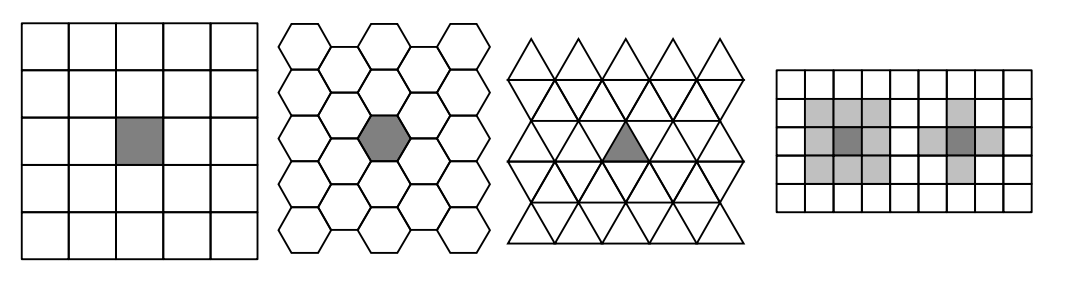
\includegraphics[width=10cm]{2_ZA_Beispiel.PNG}
\caption{Beispiele zweidimensionale zelluläre Automaten, Quelle \cite{book:bungartz}, S. 181.}
\end{figure}

Was hat nun dieses Konzept mit Verkehrsproblemen bzw. -planung zu tun? Um das zu beantworten, kann man zunächst den einfachsten Fall betrachten: Einen einspurigen Straßenabschnitt. Weiterhin nehmen wir an, dass das System abgeschlossen ist. Das bedeutet, dass jedes Auto, welches am einen Ende der Fahrbahn hinaus fährt, beim anderen Ende wieder hinein fährt. Außerdem fahren alle Fahrzeuge in die gleiche Richtung. \\

Unterteilen wir nun diesen Straßenabschnitt in mehrere Zellen erhalten wir unseren Zellraum. Eine Zelle stellt also einen Teilabschnitte des gesamten Straßenabschnittes da. Die Größe der Zellen richtet sich beispielsweise nach dem Platz den ein Auto, mit Abstand zum Fahrzeug vor ihm, minimal benötigt. \\

Der Zustandsraum umfasst die Geschwindigkeiten der Fahrzeuge, wobei diese in Zellen pro Zeitschritt angezeigt wird. Dadurch ist auch gleichzeitig vorgegeben wie weit ein Fahrzeug vorausschauen muss, um nicht mit anderen Autos zu kollidieren. \\

Die Bestimmung der diskreten Zeitschritte erfolgt anhand von Verkehrsdaten. Dabei wird zum einen die Größe der Zellen benötigt. Zum anderen eine realistische Maximalgeschwindigkeit, beispielsweise die Geschwindigkeitsbegrenzung in Deutschland von 50 innerorts oder 100 auf Landstraßen.  \\

Die Übergangsfunktion muss nun noch vorgeben, wie sich die Geschwindigkeit eines Fahrzeugs von einen Zeitschritt auf den anderen verändert. Dabei ist im Modell des zellulären Automaten das Beschleunigen, Bremsen und Bewegen berücksichtigt, nicht aber die Trödelwahrscheinlichkeit. Diese kommt erst im Nagelschreckenberg Algorithmus hinzu. \\

Beim Nagelschreckenberg Algorithmus wird jedes Fahrzeug nach einem Zeitschritt hinsichtlich seiner Geschwindigkeit neu betrachtet. Da unser Ziel ist, Staus zu vermeiden und gleichzeitig eine möglichst schnelle Fortbewegung zu erreichen, wird angenommen das jedes Fahrzeug genau die ihm mögliche Geschwindigkeit nutzt. Die Geschwindigkeit eines Fahrzeugs hängt also von der Anzahl der Zellen $d(i,j)$, die zwischen dem betrachteten Auto $i$ und dem vorher fahrenden Auto $j=i+1$ liegen und natürlich nach der Maximalgeschwindigkeit \( v_{max} \). Um das Modell noch realistischer zu machen, haben Schreckenberg und Nagel den Trödelfaktor eingefügt. Dieser bezieht ein, das Fahrer möglicherweise zu stark abbremsen, zu langsam beschleunigen oder einfach trotz freier Fahrt konstante Geschwindigkeit halten. Diese Wahrscheinlichkeit wird mit $p$ bezeichnet.\\ 


\begin{algorithm}[H]
 %\SetLine % For v3.9
 %\SetAlgoLined % For previous releases [?]
 \KwData{ \\
   \(v_{i}, v_{max}, d(i,j), p \) 
 }
 \KwResult{ \\
    Update für Fahrzeug $i$
 }

 %initialization\;
 \For{ \(i \in \{1, \cdots, n\}\) }{
   Beschleunigen: \(v_{i} := min\{ v_{i}+1,v_{max}\} \);
   \\Bremsen: \(v_{i} := d(i,i+1), \text{ falls } v_{i} > d(i,i+1) \);
   \\Trödeln: \(v_{i} := max\{(v_{i}-1, 0 \}  \text{ mit } p < 1 \);
   \\Bewegen: Fahrzeug $i$ um \(v_{i}\) Zellen vorwärts bewegen;
 }
 
 \caption{Nagelschreckenberg Algorithmus}
 \label{algo:nagelsberg}
\end{algorithm}



\section{Erweitertes Model für Kreuzungen} \label{sec:erwmodel}
Für die Modellierung einer Kreuzung benötigt man noch einige zusätzliche Annahmen. Unser Ziel ist es zwar mit einem Model die Realität möglichst gut abzubilden, doch muss dies im Verhältnis zur Komplexität des Models stehen. Um ein Model und dessen Ergebnisse verstehen zu können, müssen Bedingungen hinzugefügt werden, die nicht immer identisch mit der Realität sind. Zudem machen manche Anforderungen die Simulation in einer annehmbaren Zeit überhaupt erst möglich \\

Zunächst betrachten wir die Straße an sich. Es handelt sich um zwei einspurige Ringstraßen, welche eine Zelle gemeinsam haben. Diese Zelle ist der Kreuzungspunkt der Straßen. Bildlich beschrieben kann man sich die Straßen auch bei der Modellierung als Kreuz vorstellen. Die Autos der einen Ringstraße können nur von links nach rechts fahren, die der anderen Straße nur von unten nach oben. Den Fahrzeugen ist es nicht möglich rückwärts oder nebeneinander zu fahren. Dadurch werden auch Überholvorgänge nicht abgebildet. Zudem wird der Zellraum als abgeschlossenes System betrachtet. Ein Verlassen der Straßen ist also nicht möglich. Fahrzeuge, die sich in der obersten Zelle bzw. in der Zelle ganz rechts befinden, setzen ihren Weg in der untersten Zelle bzw. in der Zelle ganz links fort. \\

Nun müssen noch Regelungen für die Kreuzungszelle gefunden werden. Dabei werden drei Kreuzungstypen unterschieden \cite{book:bungartz}:
\begin{itemize}
	\item ungeregelte Kreuzung
      \item Kreisverkehr
      \item Kreuzungen mit geregelter Vorfahrt
\end{itemize}

Bei dem vorliegenden Model handelt es sich um eine ungeregelte Kreuzung. Es gilt also die Regel \glqq Rechts-vor-Links\grqq. Es gibt recht einfache Modelle, die die Regelung einer ungeregelten Kreuzung angeben, wie beispielsweise das Vier-Phasen-Modell. Dieses verhindert auch das Auftreten von Deadlocks, welche entstehen können wenn von allen vier Seiten gleichzeitig Fahrzeuge auf die Kreuzung zufahren. Da die Straßen in unserem Model jedoch nur einspurig ist, ergibt sich daraus eine einfache Regelung für die Vorfahrt: Die Fahrzeuge, die auf der vertikalen Straße fahren haben immer Vorfahrt. \\

Nun haben wir eine Regelung der Vorfahrt. Wie steht es allerdings mit der Geschwindigkeit auf und vor der Kreuzung? Betrachtet man die Realität, müssen Autos vor einer Kreuzung abbremsen, um nach vorfahrtsberechtigten Fahrzeugen Ausschau zu halten. Deshalb wurde in unserem Modell angenommen, dass jedes Fahrzeug vor der Kreuzungszelle auf die Maximalgeschwindigkeit von 1 Zelle pro Zeitschritt bremsen muss. Erst danach kann wieder beschleunigt werden, falls die Kreuzung frei ist. 

% - Nagelschreckenberg standard model
% - Erweitertes Model ( Das erweiterete model für Kreuzung )
\chapter{Simulationsprogramm}
Zur Bewältigung der in Kapitel \ref{sec:aufgabenstellung} beschriebenen
Aufgaben wurde das erweiterte Nagelschreckenberg Model \see{sec:erwmodel}
durch ein Matlabskript umgesetzt. Im folgenden wird dieses
Programm besprochen.

\section{Programmbedienung}
TODO beschreibung der Programmfunktionalität (buttons anzeigen etc.)

\section{Implementierung}
Von Beginn an wurde bei der Umsetzung darauf geachtet, wo immer es möglich 
war, auf Schleifen zu verzichten und stattdessen die in Matlab sehr effizient 
umgesetzten Matrixoperationen zu benutzen. Dies bedeutet vor allem, dass als 
grundlegende Datenstruktur Matrizen zu benutzen sind. 

\subsection{Die Daten: Kreuzung, Straße und Auto}
Eine Kreuzung besteht aus zwei Straßen, welche zur Vereinfachung als Horizontale und Vertikale
bezeichnet werden. Beide Straßen haben den Kreuzungspunkt als gemeinsamen Straßenabschnitt. Dieser
wird zweimal, in der Horizontalen und in der Vertikalen, abgespeichert. 
Weiter muss die Verkehrssitation für jeden Zeitpunkt abgespeichert werden und
es sollen Autos langsam an den Kreuzungspunkt heranfahren. 
Für eine Straße werden demnach die folgenden Daten benötigt:
\begin{enumerate}
  \item Anzahl der Zellen \(N \in \mathbb{N}\)
  \item Anzahl der Zeitschritte die Simuliert werden \(T \in \mathbb{N}\)
  \item Koordinate des Kreuzungspunktes \(c \in \{ 1, \ldots N \}\)
\end{enumerate}
Die Koordinaten entsprechen dabei den Zellennummern (von links nach rechts, bzw. unten nach oben vortlaufend durchnummeriert). Was noch fehlt sind die Fahrzeuge selbst. Diese werden zu einem festen Zeitschritt beschrieben druch:
\begin{enumerate}
  \item Autonummer \(k \in \{ 1, \ldots, K \}, \; K \leq N\) 
  \item Geschwindigkeit \(v_k \in \{0, \ldots, v_{max} \}\)
  \item Position, d.h. Straße und Zellenkoordinate
\end{enumerate}
Dabei ist die Autonummer nur innerhalb einer Straße eindeutig. Dies ist ausreichend, da die Fahrzeuge nicht 
abbiegen, d.h. eine Straße nicht verlassen.

Insgesamt wird eine Straße durch zwei \(T \times N\)-Matrizen \(V, W\) beschrieben.
Die \(t\)-te Zeile dieser Matrizen stellt die Situation zur Zeit \(t\) (mit \(1 \leq t \leq T\)) dar, 
wobei die Spalten den Zellen entsprechen in denen ein Auto stehen kann. 
Steht also zur Zeit \(t\) das Auto mit Nummer \(k\) (mit \(1 \leq k \leq K\)) und Geschwindigkeit \(v_k\) in der \(n\)-ten Zelle, 
so so gilt \( W_{t, n} = k\) und \(V_{t, n} = v_k\). 
Ist andererseits zur Zeit \(t\) die \(n\)-te Zelle nicht belegt so gilt: \(W_{t, n} = 0 = V_{t, n}\).
Kurz gesagt \(V\) speichert die Geschwindigkeiten und \(W\) die Autonummern zu jeder Stelle und jedem Zeitpunkt.

Zu Beginn ist nur die jeweils erste Zeile, d.h. der erste Zeitschritt, initialisiert und die anderen Matrixeinträge
sind mit Null vorbelegt. Dabei werden die Autos mit zufälliger Position und Geschwindigkeit gemäß
einer eingestellten Dichte \(\rho\) gesetzt. Dies erledigt die Funktion \code{init\_street.m} \footnote{Die tatsächliche 
Implementierung ist etwas allgemeiner. So können beispielsweise mehrere Kreuzungen und auch andere
Hindernisse eingebaut werden, an dennen Autos nur mit Geschwindigkeit \(1\) vorbeifahren können. Der Rest des Programms 
beschränkt sich jedoch auf den Spezialfall einer Kreuzung.}:
\begin{enumerate}
  \item Übergabeparameter
    \begin{enumerate}
      \item Anzahl der Zellen bis zur Kreuzung \(n\) 
      \item Verkehrsdichte \(\rho\)
      \item Simulationsdauer \(T\)
      \item Höchstgeschwindigkeit \(v_{max}\) 
    \end{enumerate}
  \item Rückgabewerte
    \begin{enumerate}
      \item Koordinate der Kreuzung \(c\) 
      \item Geschwindigkeitsmatrix \(V\) von Dimension \(T \times N\) \\ mit \(N := 2n+1\)
      \item Autonummernmatrix \(W\) von Dimension \(T \times N\) 
    \end{enumerate}
\end{enumerate}
Die Erzeugte Straße ist also \(2n+1\) Zellen lang und der Kreuzungspunkt befindet sich  in der Mitte, d.h. an der 
Koordinate \(c = n+1\). Im weiteren Programmverlauf wird jedoch nur der Rückgabewert \(c\) ausgwertet, so dass die Kreuzung
leicht verschoben werden kann. Hier ein Beispiel für \(n=2\) und \(T=2\):
\[
  V = 
  \begin{bmatrix}
    v_1& 0& 0& v_2& v_3 \\
    0& 0& 0& 0& 0
  \end{bmatrix}, \;
  W = 
  \begin{bmatrix}
    1& 0& 0& 2& 3 \\
    0& 0& 0& 0& 0
  \end{bmatrix}, \;
  c = 3
\]
Es stellt sich die Frage, ob man auch mit einer Matrix auskommt. Eine Möglichkeit besteht darin sich nur die Geschwindigkeitsmatrix 
zu speichern und freie Straßenabschnitte mit \(-1\) zu kodieren. Dann ist es jedoch nicht ohne Weiteres möglich den Zustand eines bestimmten Autos über
mehrere Zeitschritte hinweg zu verfolgen, vorallem wenn zukünftige Erweiterungen beispielsweise Überholmanöver der Autos erlauben sollen.

\subsection{Der Algorithmus: Beschleunigen, Bremsen und Trödeln}
Wir betrachten zunächst die Vertikale und die Horizontale getrennt, d.h. das Folgende wird
auf beide Straßen angewendet.

Um den nächsten Zeitschritt berechnen zu können muss man zunächst für jedes Auto wissen, wie viele freie Zellen 
in Fahrtrichtung vorhanden sind. Dabei reicht es \(v_{max}\) Zellen vorauszuschauen. 
Eine Zelle ist genau dann nicht frei, wenn sie ein Auto beinhaltet oder
die Kreuzungszelle ist. Hierfür wurde die Funktion \code{freeCells.m} geschrieben:
\begin{enumerate}
  \item Übergabeparameter
    \begin{enumerate}
      \item Straßenbelegung \(w_t\) zum Zeitpunkt \(t\),  also die Zeile \(t\) der Matrix \(W\)       
      \item Koordinate der Kreuzung \(c\) 
      \item Maximale Geschindigkeit \(v_{max}\)
    \end{enumerate}
  \item Rückgabewerte
    \begin{enumerate}
      \item Vektor \(u\) der Länge \(N\) mit \(u_i \in \{0, \ldots, v_{max} \}\) ist Anzahl der freien 
        Zellen in Fahrtrichtung ab Zelle \(i\), also \(j := i + u_i + 1 \Rightarrow W_{t,j} \neq 0 \lor j = c\).
    \end{enumerate}
\end{enumerate}
Nun kann entsprechend Gebremst oder Beschleunigt werden. So wird für alle mit Autos belegten Zellen \(i\)
die neue Geschwindigkeit auf \(u_i\) gesetzt falls \(u_i < v\) und auf \(v\) falls \(u_i \geq v\) mit
\( v := \min\{ v_{max}, V_{t,i}+1 \}\).  
Dafür wurde die Funktion \code{adjustSpeed.m} geschaffen, die intern \code{freeCells.m} benutzt:
\begin{enumerate}
  \item Übergabeparameter
    \begin{enumerate}
      \item Straßenbelegung \(w_t\) zum Zeitpunkt \(t\),  also die Zeile \(t\) der Matrix \(W\)       
      \item Geschwindigkeiten \(v_t\) zum Zeitpunkt \(t\),  also die Zeile \(t\) der Matrix \(V\)       
      \item Koordinate der Kreuzung \(c\) 
      \item Maximale Geschindigkeit \(v_{max}\)
    \end{enumerate}
  \item Rückgabewerte
    \begin{enumerate}
      \item Vektor \(\hat{v}\) der Länge \(N\) mit \(\hat{v}_i\) ist neue Geschwindigkeit des Autos der Zelle \(i\)
    \end{enumerate}
\end{enumerate}
Insbesondere bleiben Autos zunächst vor der Kreuzung stehen. Nach dem Aufruf von \code{adjustSpeed.m} für die
Horizontale und die Vertikale kann also entschieden werden ob ein Auto den Kreuzungspunkt betretten darf. 
Dazu wird überprüft ob die Kreuzung frei. Es bezeichne \(W^h\), \(\hat{v}^h\) und \(c^h\) 
die Autonummernmatrix, den angepassten Geschwindigkeitsvektor und den Kreuzungspunkt der Horizontalen, sowie
\(W^v\), \(\hat{v}^v\), \(c^v\) das selbige für die Vertikale. Ist die Kreuzung frei so muss demnach gelten: 
\[W^h_{t,c^h} = 0 = W^v_{t,c^v}\] 
Ist dies der Fall und steht auf der Vertikalen
ein Auto vor der Kreuzung 
\[W^v_{t,c^v-1} \neq 0\] so darf dieses Auto über die Kreuzung mit Geschwindigkeit \(1\). 
Es wird also 
\[\hat{v}^v_{c^v-1} = 1\] 
gesetzt. Steht auf der Vertikalen kein Auto for der Kreuzung, 
aber auf der Horizontalen 
\[W^h_{t,c^h-1} \neq 0\]
so wird dessen angepasste Geschwindigkeit auf \(1\) gesetzt. 
Damit ist die Regel \textit{Rechts vor Links} umgesetzt.

Hiernach wird für beide Straßen einzeln getrödelt (\code{linger.m}), also mit einer festgesetzten Wahrscheinlichkeit werden
die Geschwindigkeiten in \(\hat{v}\) um eine Einheit reduziert. 
Schließlich erfolgt durch die Funktion \code{shift.m} für beide Straßen einzeln die Berechnung des nächsten Zeitschrittes, 
also der Zeile \(t+1\) in den Matrizen \(V,W\) gemäß der Geschwindigkeiten \(\hat{v}\).

Der hier beschriebene Vorgang zur Berechnung der Zeitschritte ist in der Funktion \code{nagelschreckenberg.m} umgesetzt, 
sodass über die oben beschriebene GUI mit verschiedenen Startbedingungen (z.B. Trödelwahrscheinlichkeiten, Verkehrsdichten, Streckenlängen) experimentiert werden kann.



% - Beschreibung des Programms (der Funktionalität! ... evtl. hier überschneidung mit vorherigem)
% - Beschreibung der programmtechnischen Umsetzung
\chapter{Ergebnisse}
TODO bildchen uns zeug (Plot des fundamental diagramms für
verschiedene dichteeinstellungen etc...)



% - Simulations bildchen und ergebnisse darstellen
% - Bedeutung des Fundamentaldiagrammes erklären, erwähnen dass unsere Version ein Spezialfall der im Bungartz dargestellten Variante ist. 
\chapter{Fazit}

Fazit: Ziel unserer Simulation war es, Hinweise auf den maximalen Verkehrsfluss auf beiden Straßen zu bestimmen. Dazu wollen wir den gesamten Fluss bestimmen, dies ist einfach die Summe aus den beiden einzelnen Verkehrsflüssen.\\

Der Verkehrsfluss der horizontalen Straße hängt im wesentlichen von der Dichte der vertikalen Straße ab. Aus \cite{book:bungartz} ist bekannt, dass für eine einfache Ringstraße der Verkehrsfluss für eine Dichte von $\rho_max \approx 0.12$ maximal ist, dabei ist der Fluss $f \approx 3000$ Autos pro Stunde. Außerdem können wir aus dieser Quelle entnehmen, dass realistische Verkehrsbedingungen mit einer Trödelwahrscheinlickeit von $p=0.2$ erreicht werden. Deshalb haben wir im Folgenden die horizontale Dichte $\rho_v$ auf den Wert $0.12$ festgesetzt und sind von einer Trödelwahrscheinlichkeit $0.2$ ausgegangen. 
%
\begin{figure}[h]%
\centering
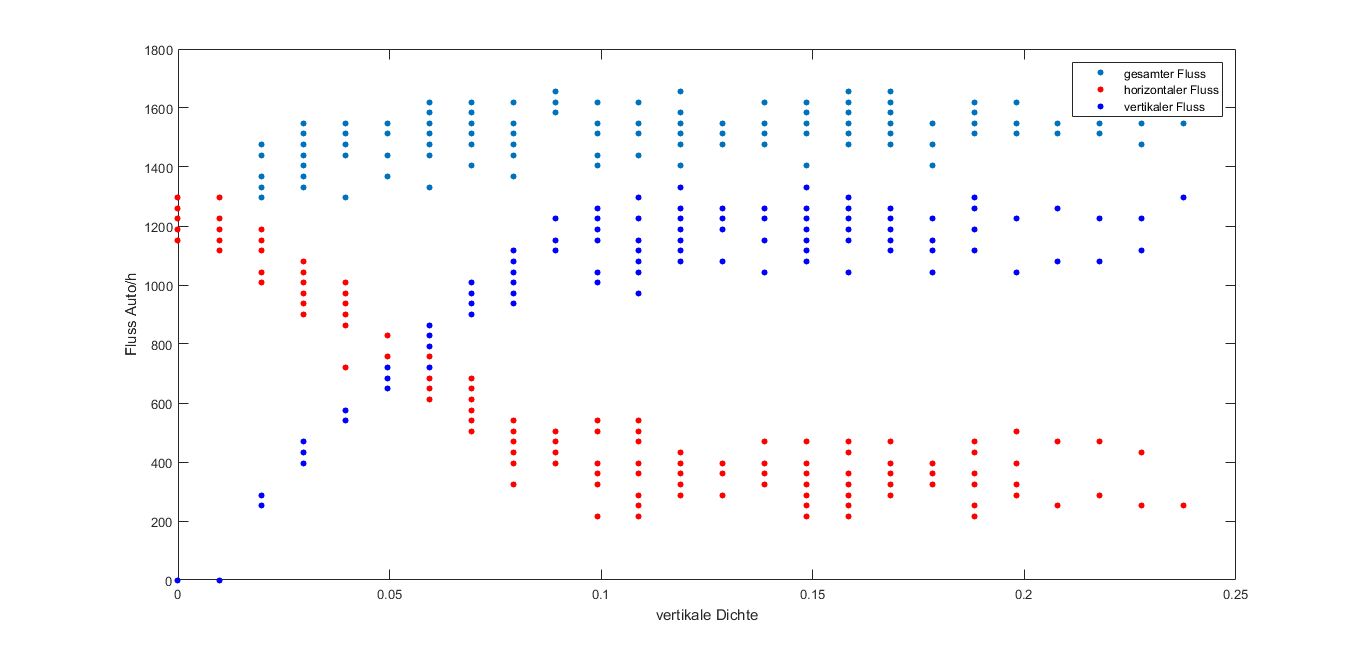
\includegraphics[width=17cm]{MaxFluss.png}%
\caption{Die verschiedenen Flüsse für $p=0.2$, $rho_h=0.12$ und einer Straßenlänge von je 300 Zellen.  }%
\label{pic:MaxFluss}%
\end{figure}
%
In der Abbildung \ref{pic:MaxFluss} sind die einzelnen Flüsse in einer Grafik dargestellt. Man kann erkennen, dass sich der gesamte Fluss im wesentlichen Konstant auf einem Niveau von ca. 1500 Autos pro Stunde hält. Ein Grund für diese Erscheinung ist die Bedingung, dass sich beide Ringstraßen eine Zelle, nämlich die Kreuzungszelle teilen. Dadurch wird der Fluss begrenzt, da jedes Auto vor der Kreuzung auf Geschwindigkeit 1 abbremst und somit jedes Auto auf der Kreuzungszelle gewesen sein muss. Durch das Abbremsen wird auch die Geschwindigkeit auf der Kreuzung limitiert, so kann ein Auto nur mit geringer Geschwindigkeit über die Kreuzung fahren.

Ausblick:\\
TODO mögliche Erweiterungen wie Ampel oder mehr Kreuzungen oder Abbiegen etc.

% - Fazit und co..

% Anhang (Screenies etc.)
%\begin{appendix}

\chapter{Anhang}

TODO hier evtl auschnitte des programmcodes ???


\end{appendix}


% Gloassar / Begriffserkläerungen
%\renewcommand{\nomname}{Begriffserklärungen}
%\label{cha:nomencl}
%\printnomenclature

% Quellenverzeichnis
\renewcommand{\bibname}{Quellenverzeichnis}
\bibliographystyle{geralpha}
\bibliography{document}

\end{document}

